% A stand-in for a source figure, in a Stata-like palette so restyle_figs.py
% has something to recolour. Build: lualatex example.tex (from figs/).
\documentclass[tikz,border=2pt]{standalone}
\usepackage{pgfplots}\pgfplotsset{compat=1.16}
\definecolor{stnavy}{HTML}{1A476F}\definecolor{stmaroon}{HTML}{90353B}\definecolor{stbg}{HTML}{EAF2F3}
\begin{document}
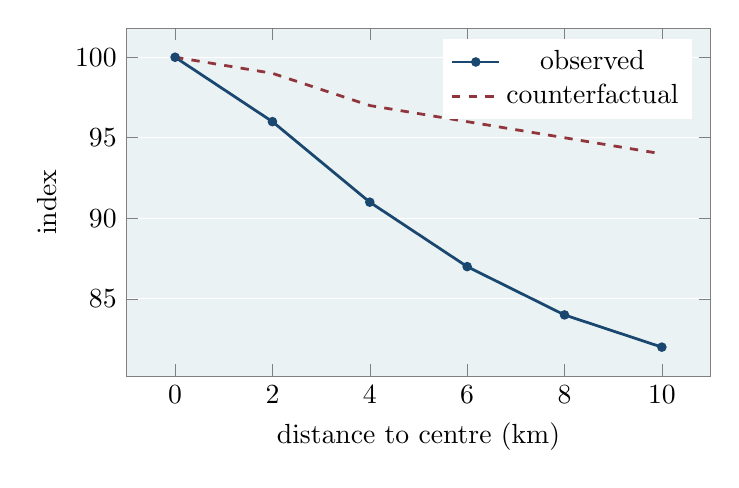
\begin{tikzpicture}
\begin{axis}[width=90mm, height=60mm, axis background/.style={fill=stbg}, xlabel={distance to centre (km)}, ylabel={index}, ymajorgrids, grid style={white}, tick style={gray}, axis line style={gray}, legend style={draw=none}, legend pos=north east]
\addplot[stnavy, line width=1pt, mark=*, mark size=1.2pt] coordinates {(0,100)(2,96)(4,91)(6,87)(8,84)(10,82)};
\addplot[stmaroon, line width=1pt, dashed] coordinates {(0,100)(2,99)(4,97)(6,96)(8,95)(10,94)};
\legend{observed, counterfactual}
\end{axis}
\end{tikzpicture}
\end{document}
